\documentclass{article}
\usepackage[utf8]{inputenc}
\usepackage{xurl}
\usepackage[czech]{babel}
\usepackage{csquotes}

\MakeOuterQuote{"}

% \setlength{\parskip}{\baselineskip}
% \setlength{\parindent}{0pt}

\title{Metody analýzy dat I - analýza datasetu}
\author{Filip Peterek, PET0342}
\date{28. prosinec 2021}

\begin{document}

\maketitle

\section{Popis datové sady}

Datová sada obsahuje seznam nahlášených zločinů za rok 2018 ve městě Austin
v americkém státě Texas. Data byla sbírána policií města Austin a následně
veřejně publikována \cite{dataset-source}. Datová sada obsahuje 37156 záznamů
odpovídajících 37156 nahlášeným zločinům.

\subsection{Atributy datové sady}

V datové sadě se objevuje 13 atributů, které jsou popsány v následující tabulce.

\begin{table}
  \centering
  \caption{Popis atributů datové sady}
  \begin{tabular}{ |l|l|l|l|l| }
  \hline
    Název & Popis & Typ & Datový typ & Povinný \\
    GO Primary Key & ID incidentu & numerický & celé číslo & ano \\
    Council District & městská čtvrť & kategoriální & celé číslo & ne \\
    GO Highest Offense & zločin & kategoriální & řetězec & ano \\
    Crime Type & typ zločinu & kategoriální & řetězec & ano \\
    GO Report Date & den nahlášení & numerický & datum & ano \\
    GO Location & místo odehrání zločinu & kategoriální & řetězec & ne \\
    GO X Coordinate & místo odehrání zločinu & numerický & desetinné číslo & ne \\
    GO Y Coordinate & místo odehrání zločinu & numerický & desetinné číslo & ne \\
    Clearance Status & stav policejního pátrání & kategoriální & řetězec & ne \\
    Clearance Date & datum vyřešení případu & numerický & datum & ne \\
    GO District & policejní sektor & kategoriální & řetězec & ano \\
    GO Location Zip & poštovní směrovací číslo & kategoriální & celé číslo & ne \\
    GO Census Tract & čtvrť podle počtu obyvatel & kategoriální & desetinné číslo & ne \\
  \hline
  \end{tabular}
\end{table}

\section{Výsledky analýzy}

\subsection{Počty zločinů}

Počty jednotlivých zločinů \ref{fig:crime_counts} jistě nijak zarážející nejsou. Naprosto
převažují krádeže, v tomto případě se z velké části pravděpodobně jedná hlavně o kapsářství
a podobné drobné krádeže. Počet vloupání do domu je oproti obyčejným kráděžím méně
než pětinový. Násilné činy tak časté nejsou, přesto se jich několik objevuje.

\begin{figure}
  \centering
  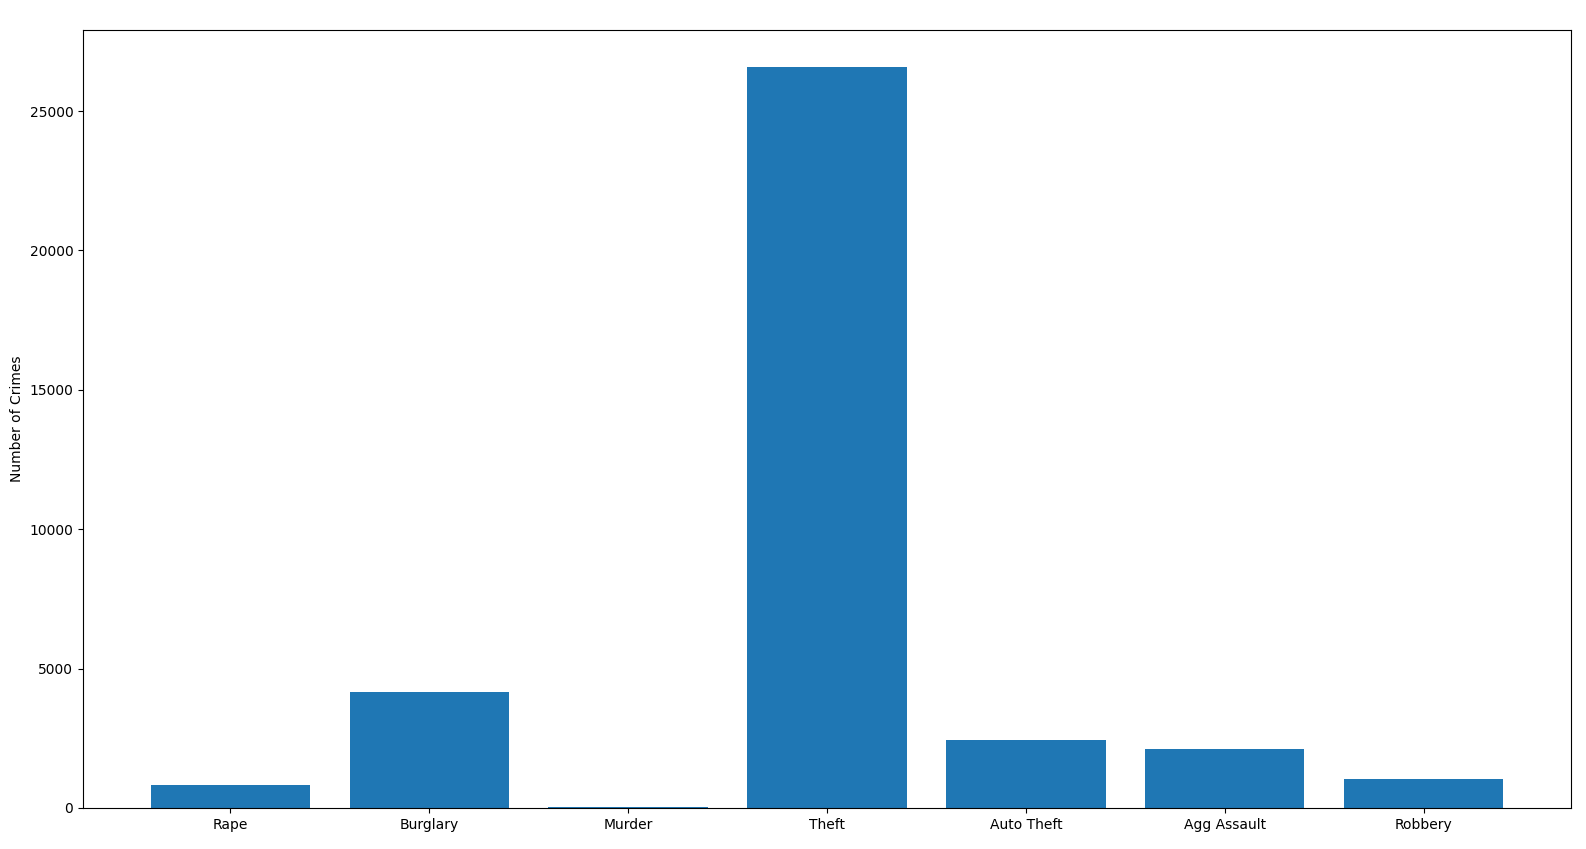
\includegraphics[width=0.9\textwidth]{figures/crime_counts.png}
  \caption{Počet nahlášených zločinů podle kategorie}
  \label{fig:crime_counts}
\end{figure}

Velmi znepokojující jsou počty nahlášeného násilí na dětech \ref{fig:crime_against_children}.
Austin je velké město, a proto se s vysokou pravděpodobností objeví zločiny všech možných typů,
přesto řádově stovky případů zneužívání dětí je alarmující číslo.

\begin{figure}
  \centering
  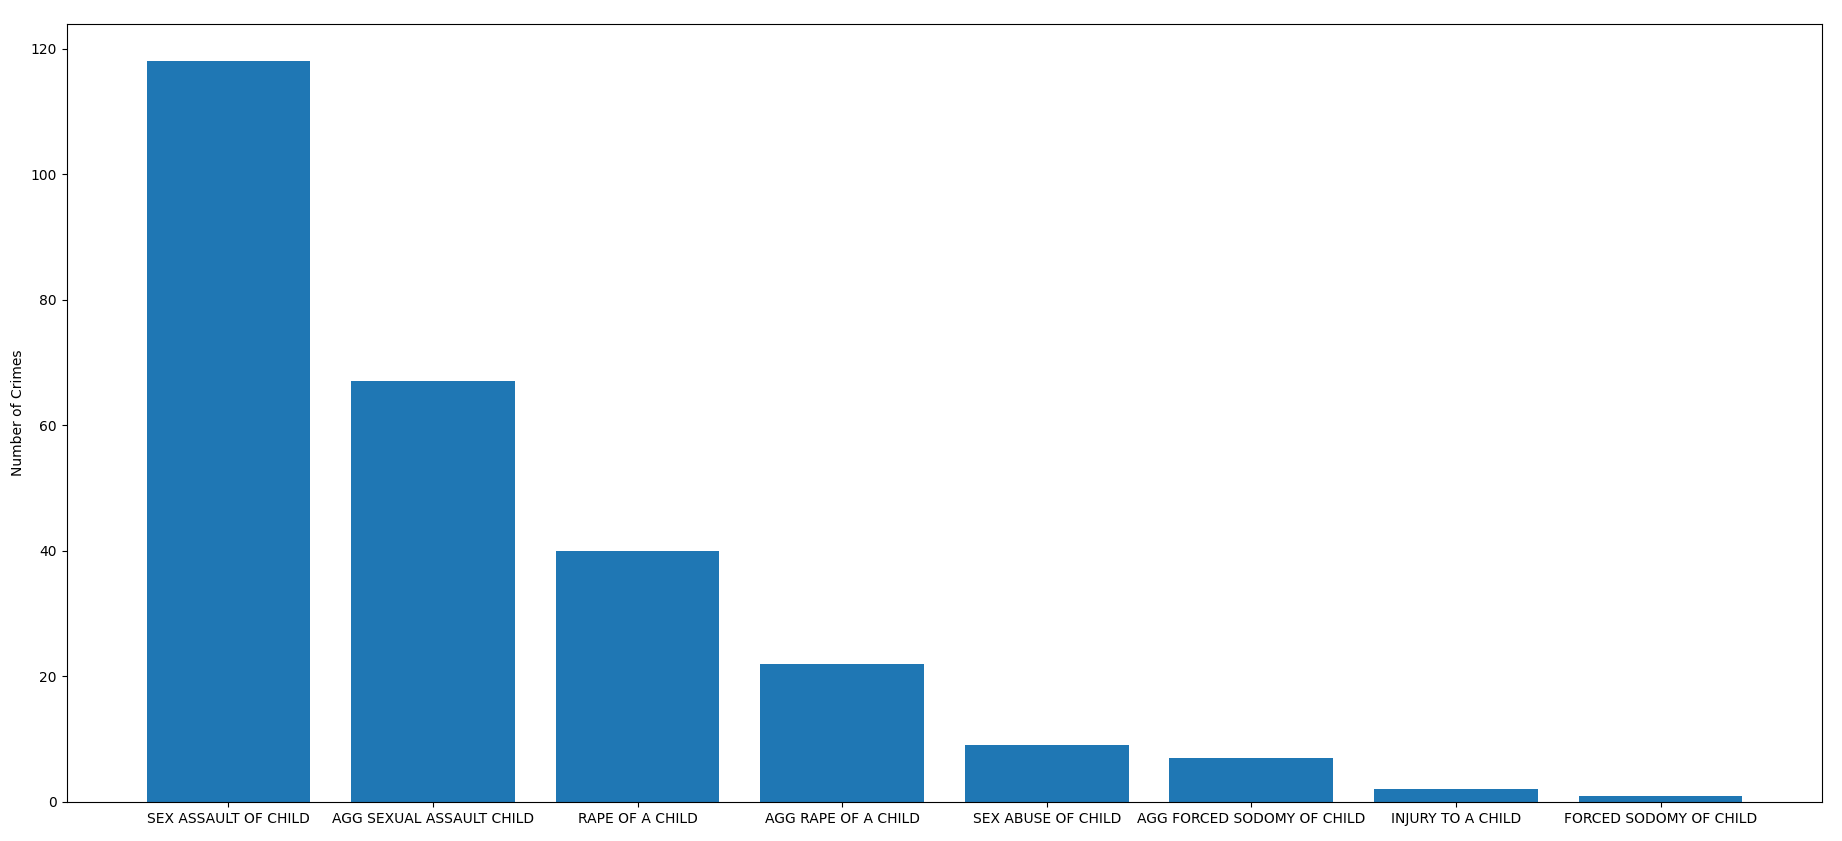
\includegraphics[width=0.9\textwidth]{figures/crime_against_children.png}
  \caption{Počet nahlášených zločinů proti dětem}
  \label{fig:crime_against_children}
\end{figure}

Počet nahlášených zločinů podle kalendářního měsíce \ref{fig:crime_per_each_month} není
nijak zajímavý. Nejméně zločinů bylo nahlášeno v únoru -- nepřekvapivě, neboť se jedná
o nejkratší měsíc v roce. Nejvíce zločinů bylo nahlášeno v říjnu. Překvapivě může působit
pouze fakt, že nedošlo k nárůstu zločinnosti v letních měsících. Austin sice nepatří
mezi nejvyhledávanější turistické destinace ve Spojených státech, přesto se však jedná
o město s bohatým kulturním vyžitím. I tak ale nedošlo k nárůstu zločinnosti v letních měsících.

\begin{figure}
  \centering
  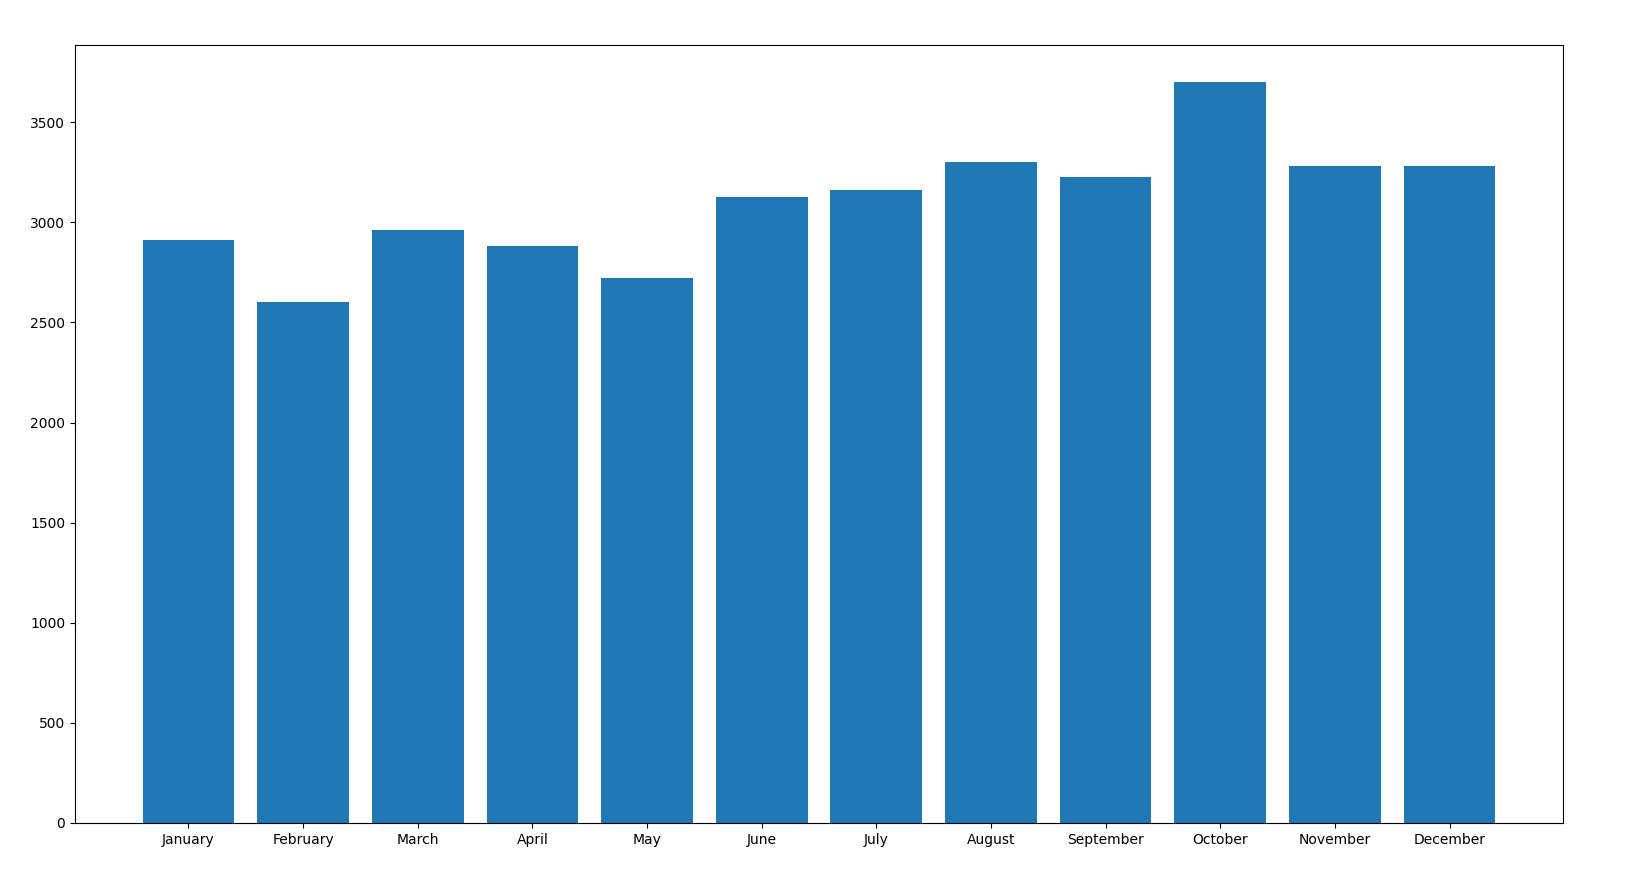
\includegraphics[width=0.9\textwidth]{figures/crime_per_each_month.png}
  \caption{Počet nahlášených zločinů podle kalendářního měsíce}
  \label{fig:crime_per_each_month}
\end{figure}

\subsection{Řešení zločinů}

Vzorného občana určitě znepokojí množství nevyřešených příkladů. Z grafu \ref{fig:clearance_status}
lze vyčíst, že naprostá většina případů zůstáva nevyřešena.

\begin{figure}
  \centering
  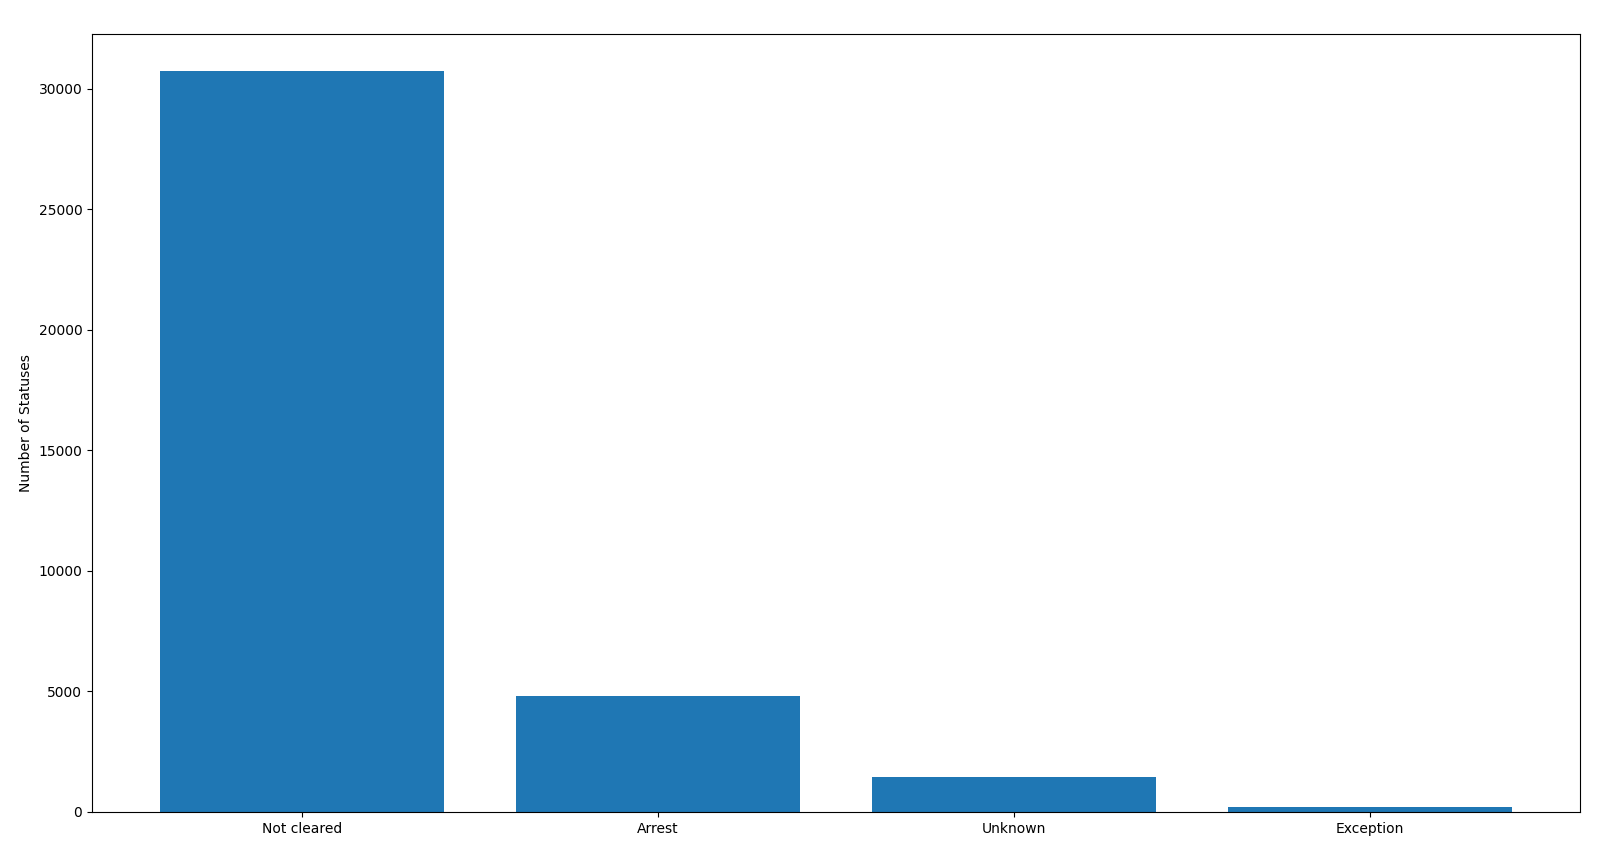
\includegraphics[width=0.9\textwidth]{figures/clearance_status.png}
  \caption{Četnosti statusů policejního pátrání}
  \label{fig:clearance_status}
\end{figure}

Vzorného občana určitě znepokojí množství nevyřešených příkladů. Z grafu \ref{fig:clearance_status}
lze vyčíst, že naprostá většina případů zůstáva nevyřešena.

\begin{figure}
  \centering
  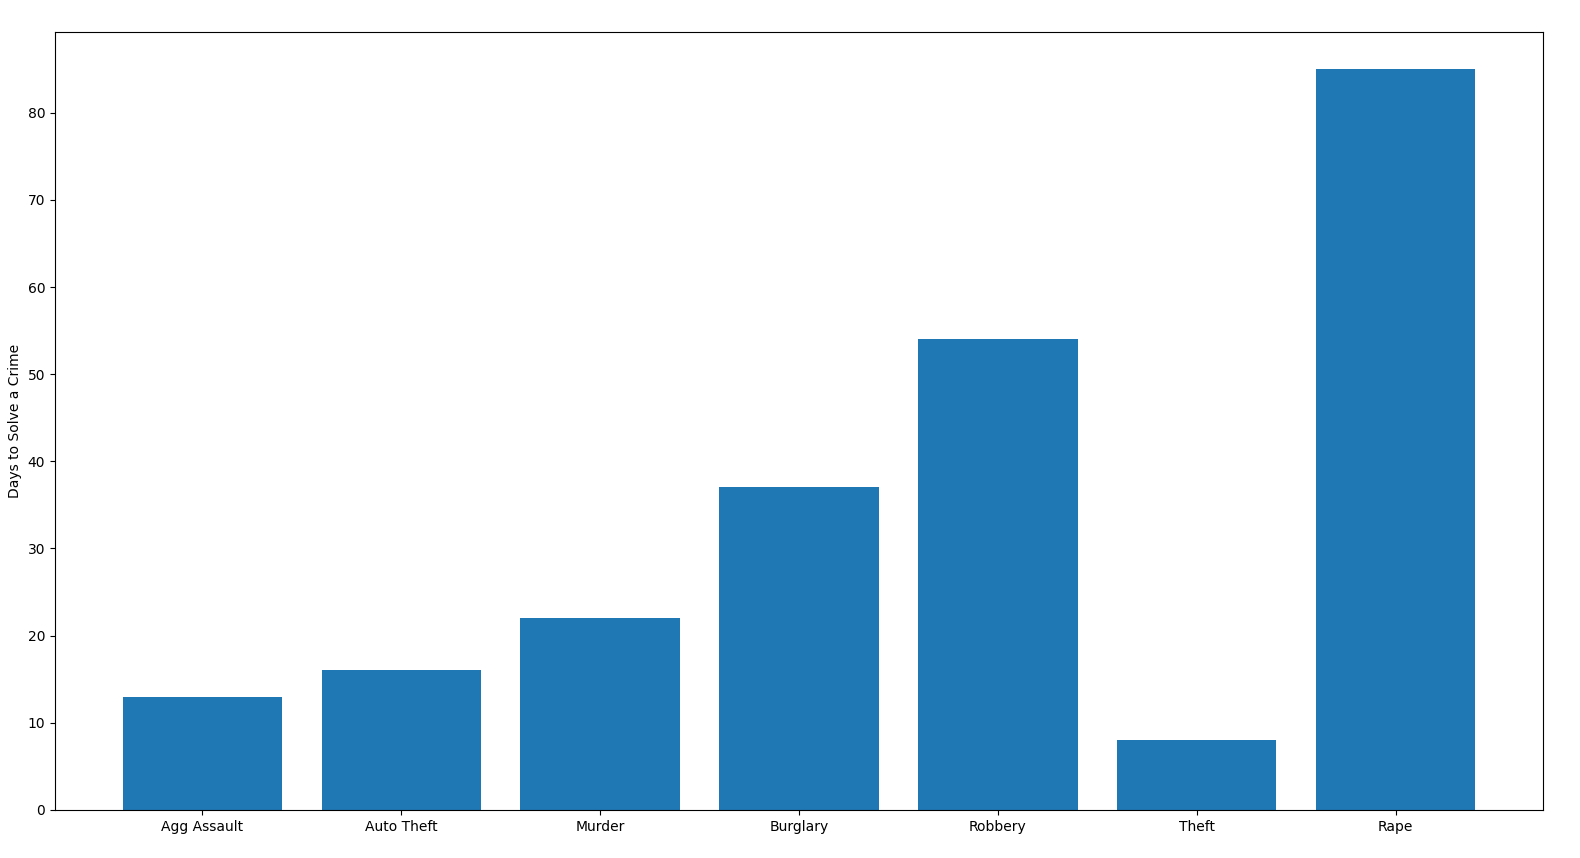
\includegraphics[width=0.9\textwidth]{figures/clearance_time.png}
  \caption{Průměrná doba úspěšného řešení}
\end{figure}

\begin{figure}
  \centering
  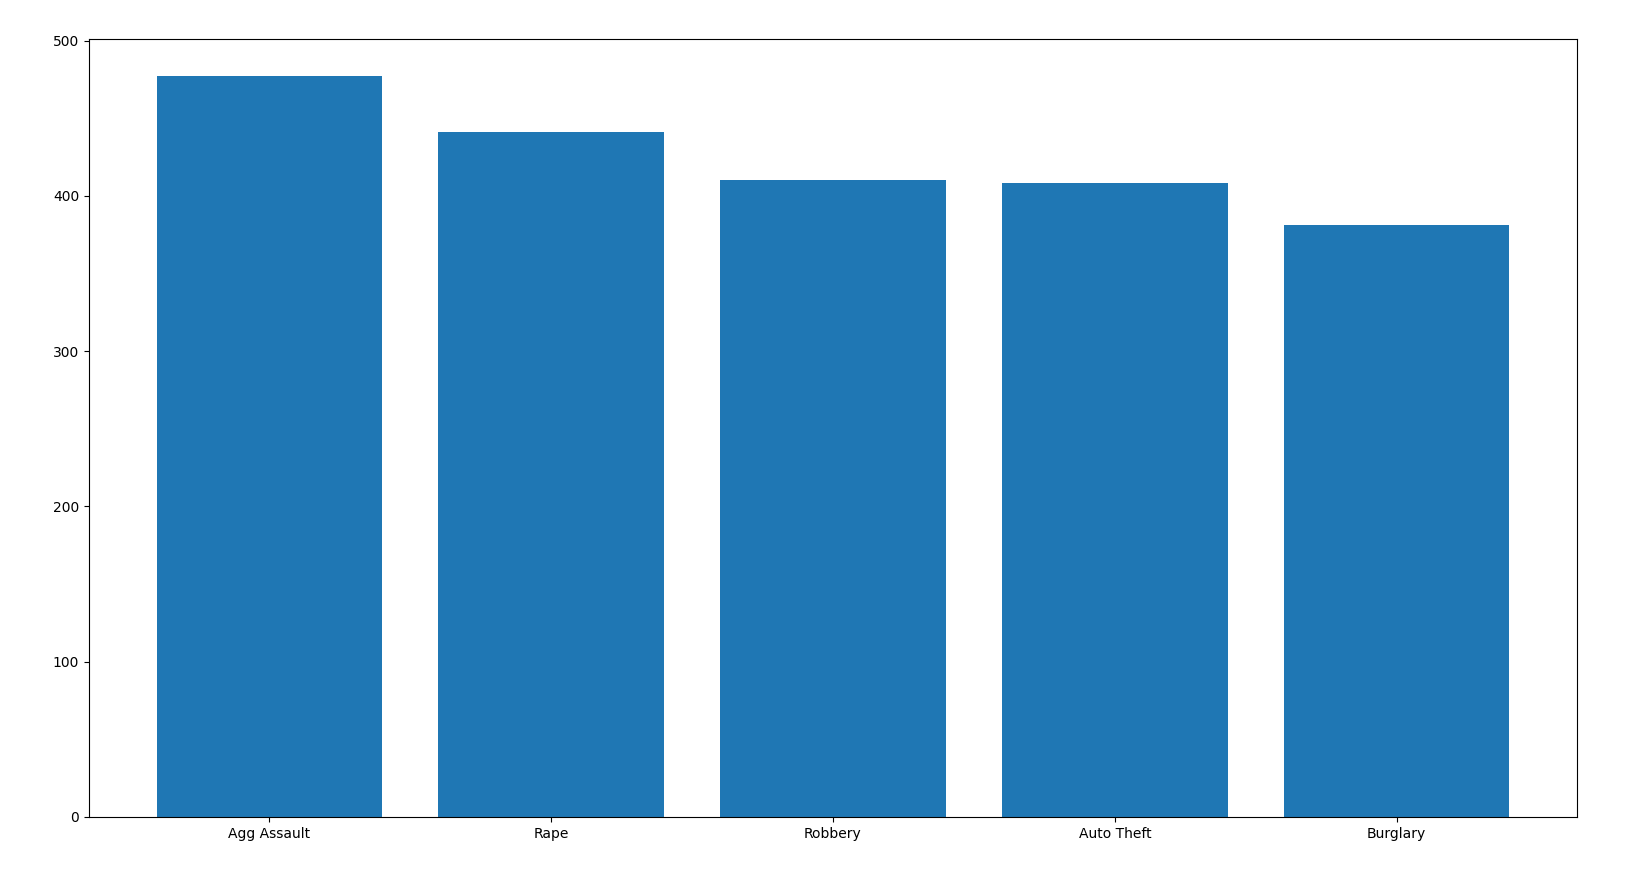
\includegraphics[width=0.9\textwidth]{figures/top_clearance_times.png}
  \caption{Nejdéle řešené jednotlivé případy}
\end{figure}

\begin{figure}
  \centering
  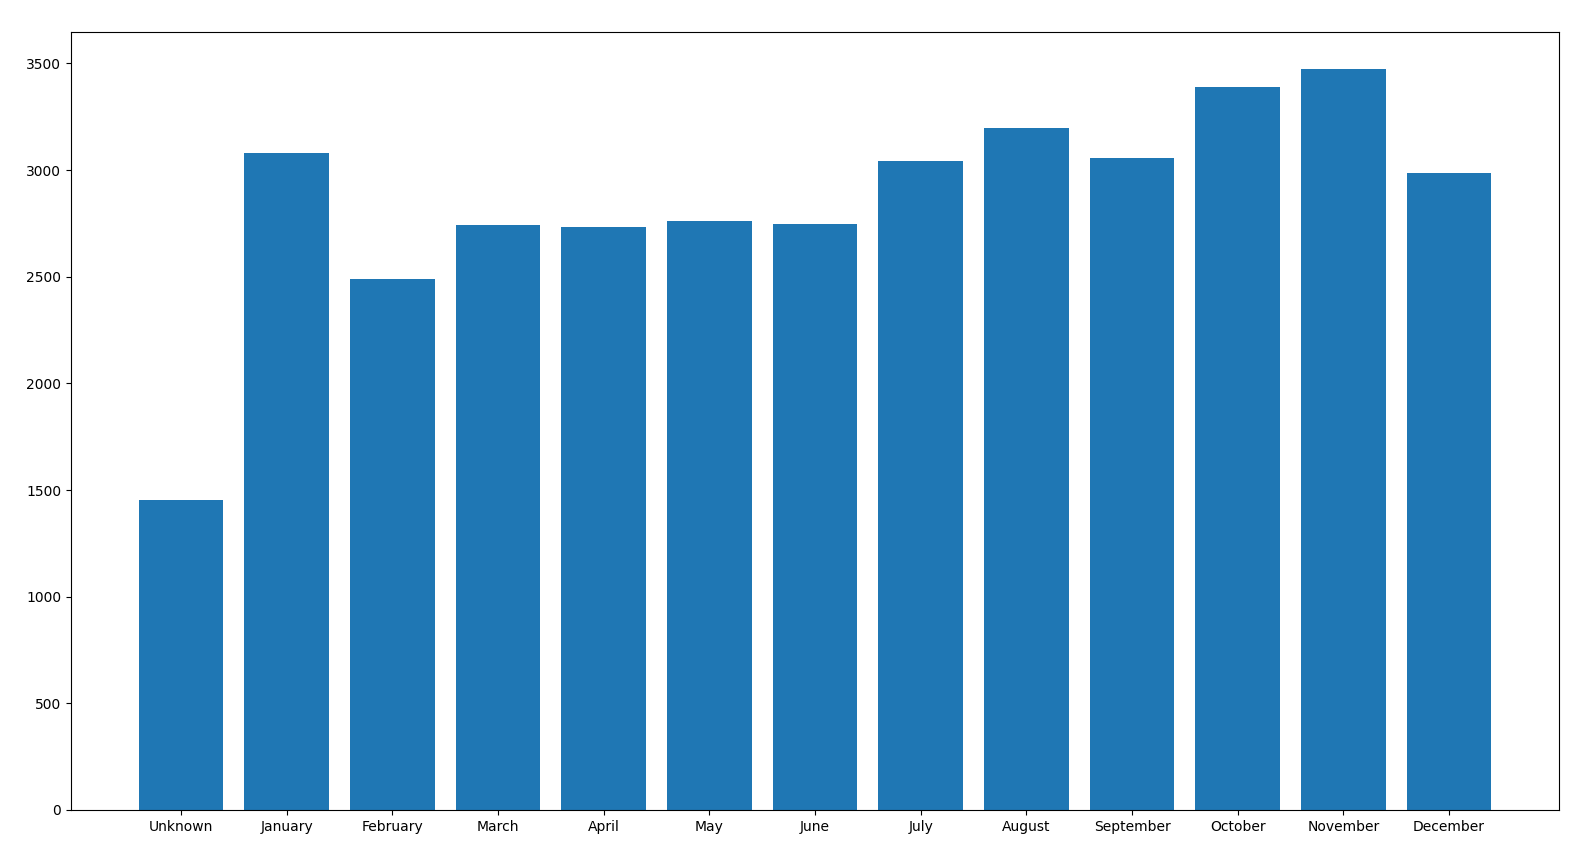
\includegraphics[width=0.9\textwidth]{figures/clearance_by_month.png}
  \caption{Počet uzavřených případů podle kalendářního měsíce}
\end{figure}

\begin{figure}
  \centering
  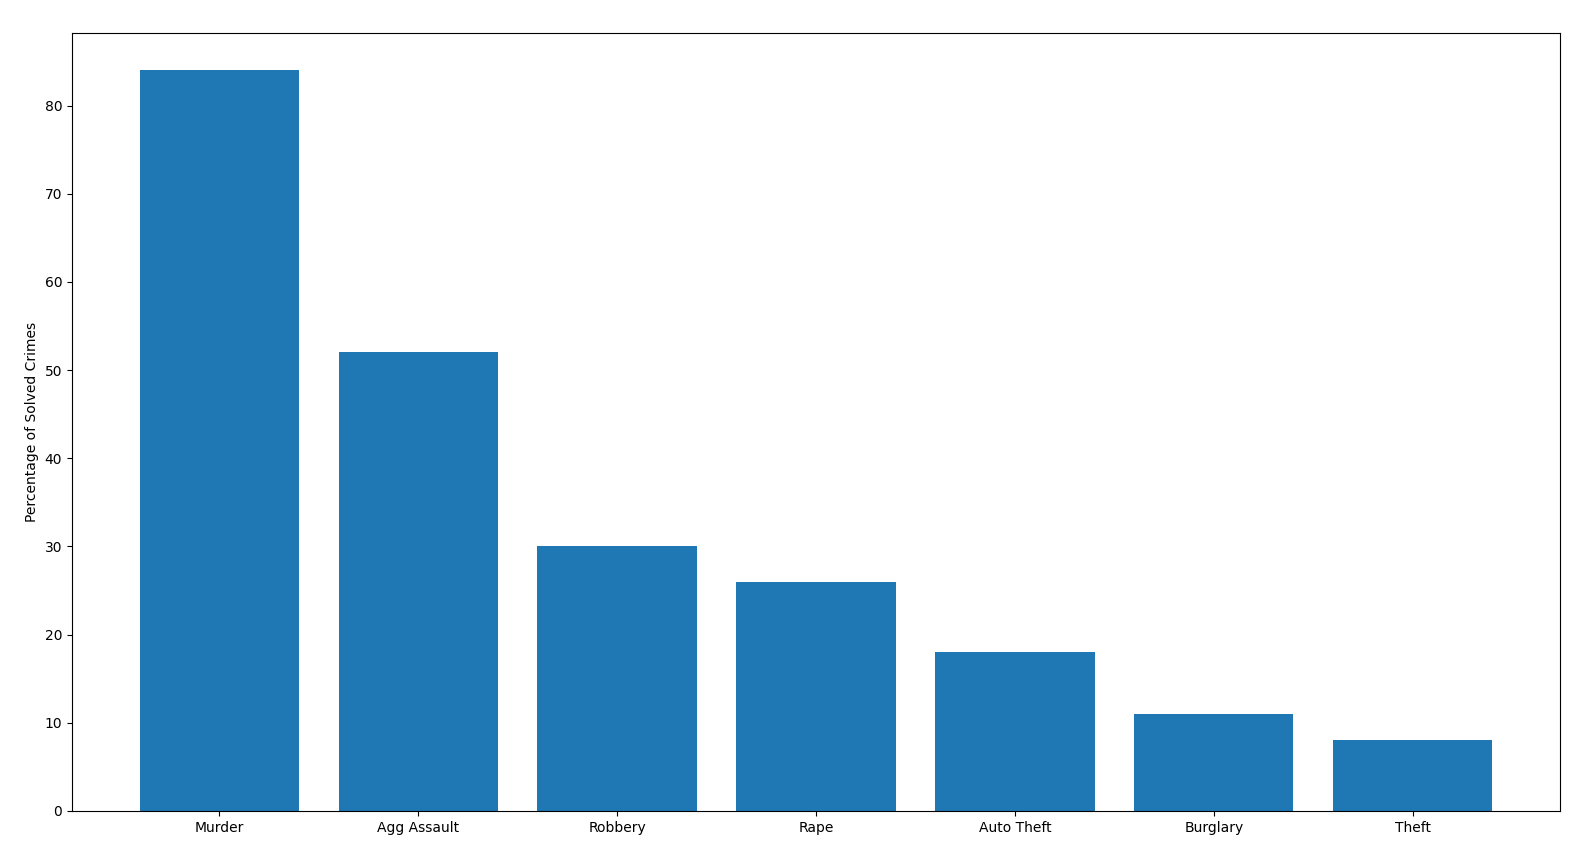
\includegraphics[width=0.9\textwidth]{figures/solved_percentage.png}
  \caption{Poměr úspěšně vyřešených případů}
\end{figure}

\subsection{Bezpečnost čtvrtí}

\begin{figure}
  \centering
  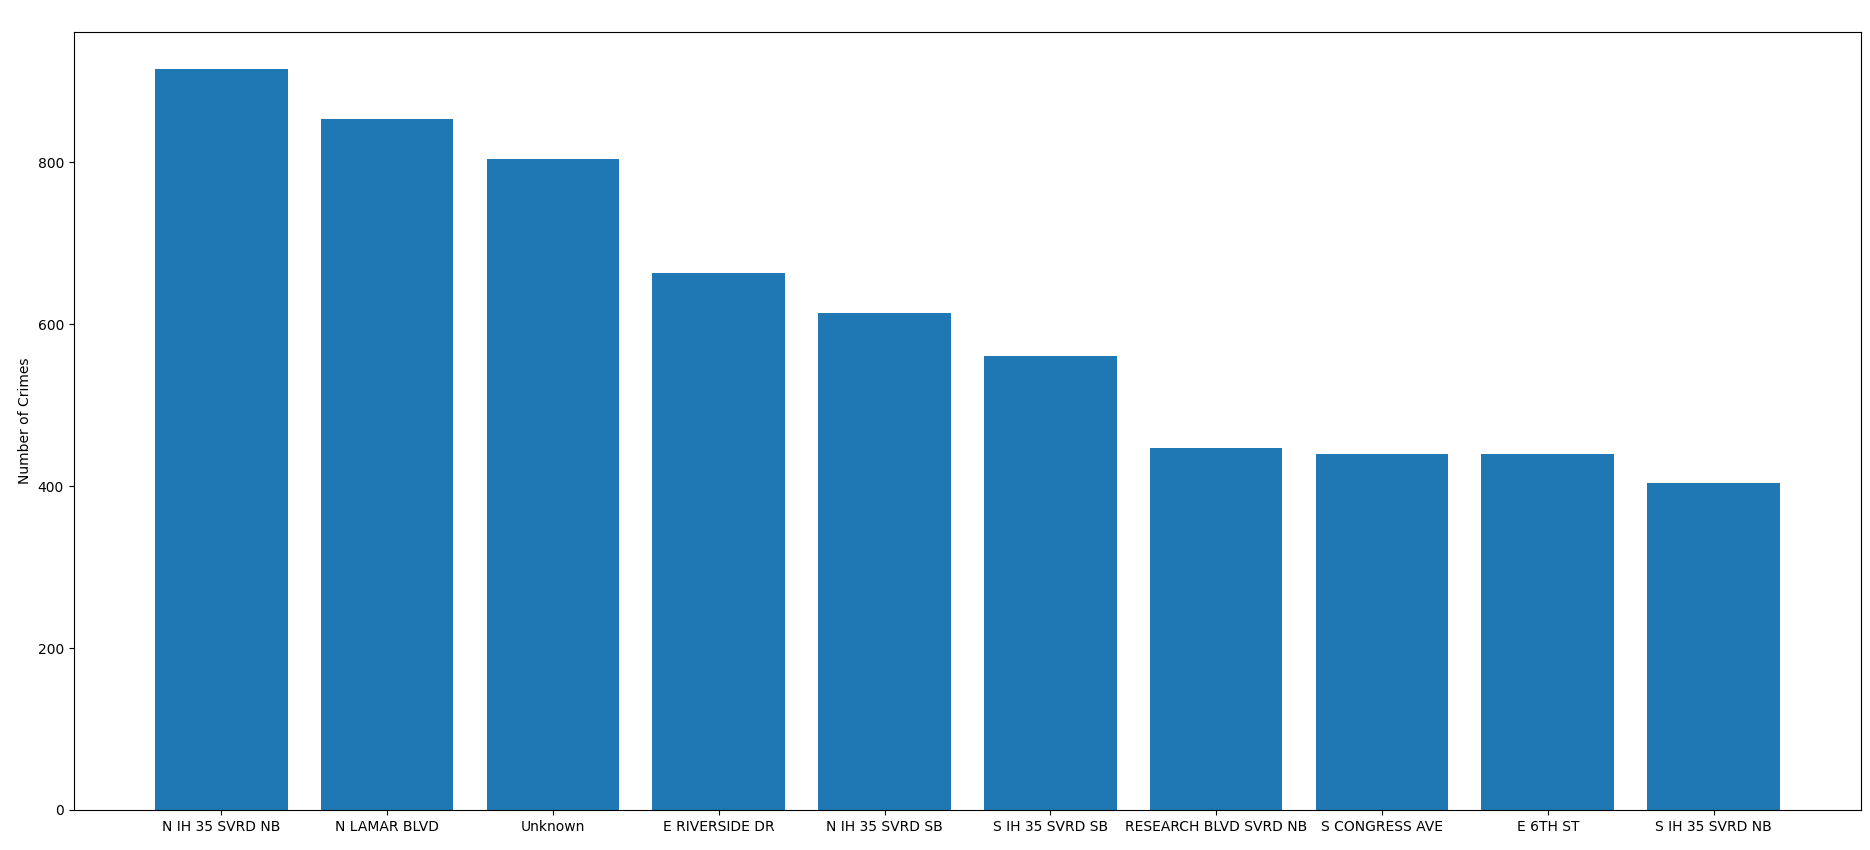
\includegraphics[width=0.9\textwidth]{figures/worst_streets.png}
  \caption{Ulice s nejvyšším počtem nahlášených zločinů}
\end{figure}

\begin{figure}
  \centering
  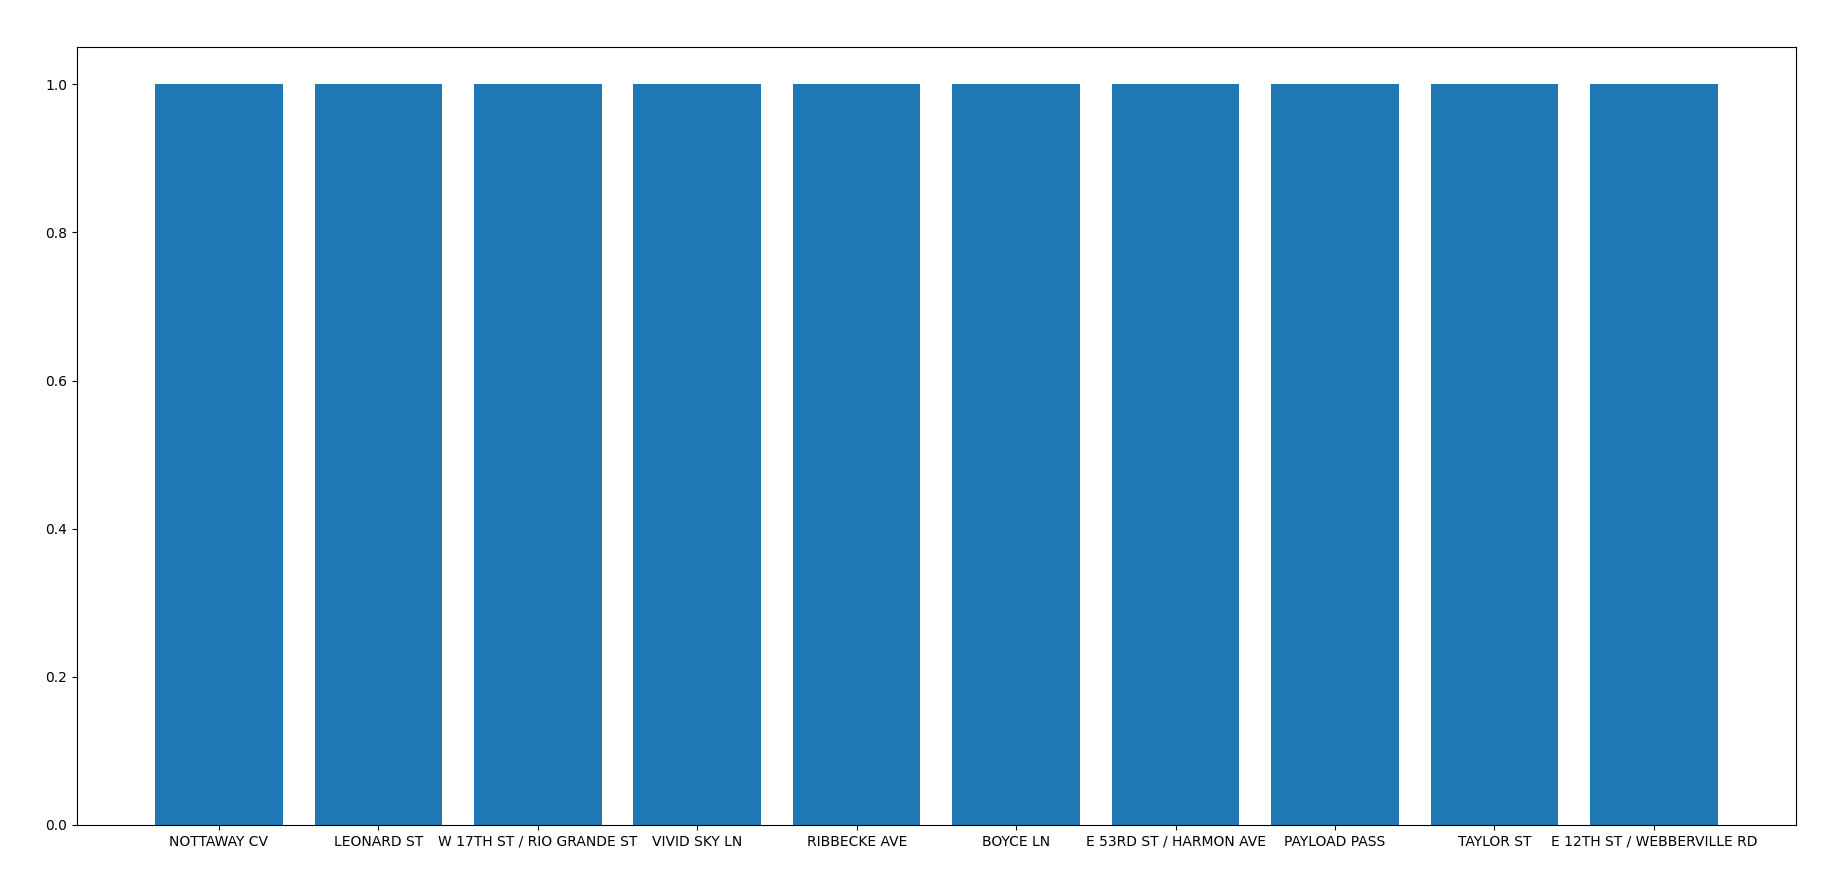
\includegraphics[width=0.9\textwidth]{figures/safest_streets.png}
  \caption{Ulice s nejnižším počtem zločinů (ulice bez zločinů jsou ignorovány)}
\end{figure}

\begin{figure}
  \centering
  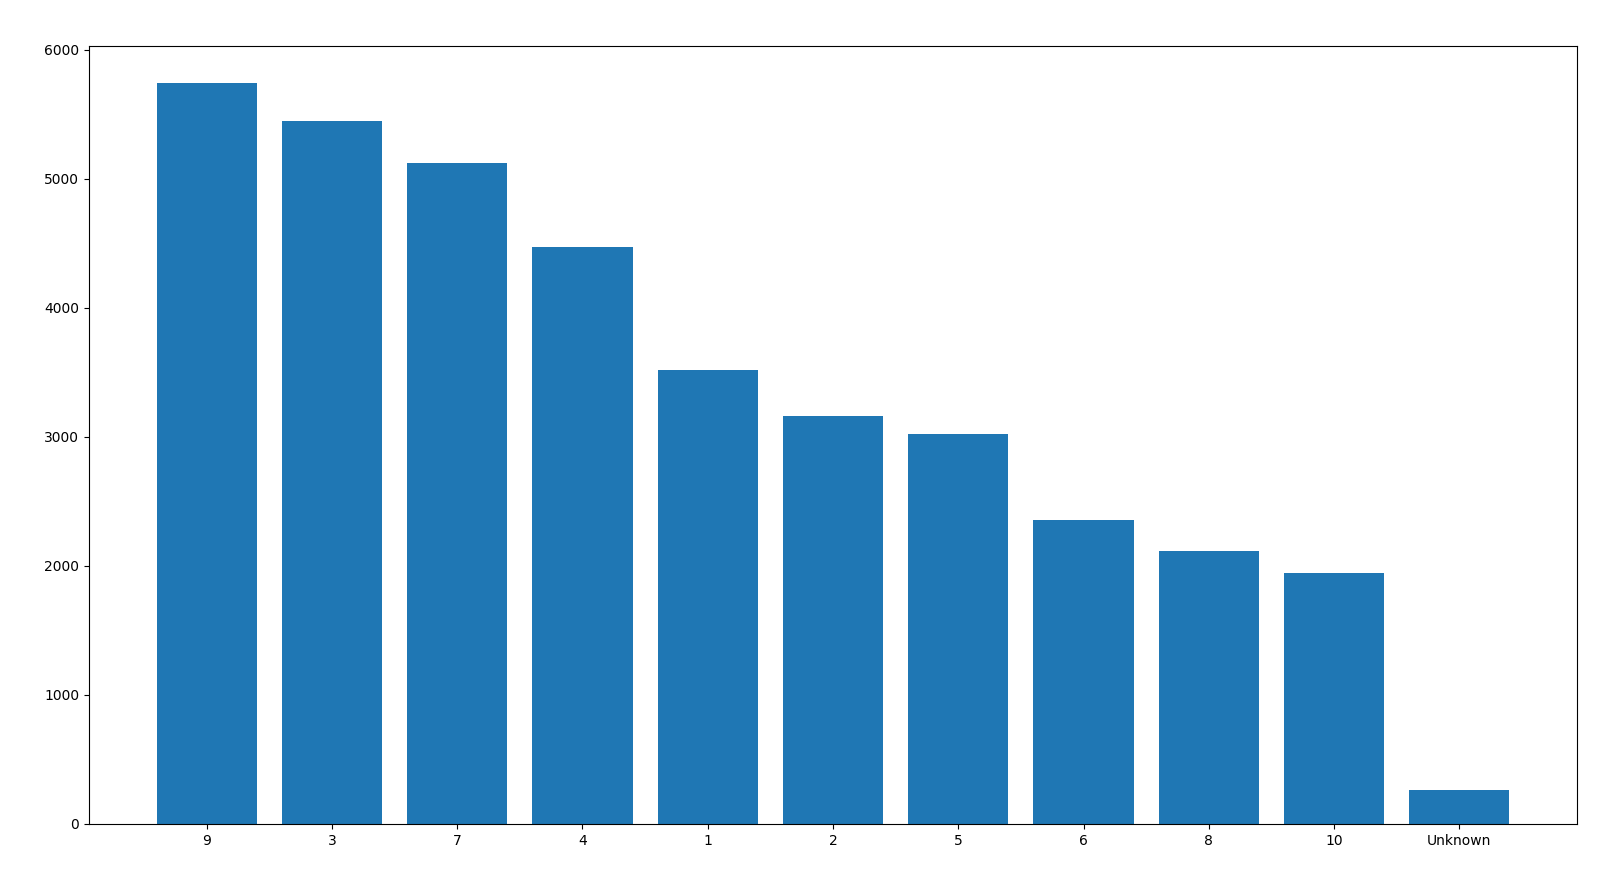
\includegraphics[width=0.9\textwidth]{figures/worst_districts.png}
  \caption{Čtvrti s nejvyšším počtem nahlášených zločinů}
\end{figure}

\subsection{Slaughter lane}

\begin{figure}
  \centering
  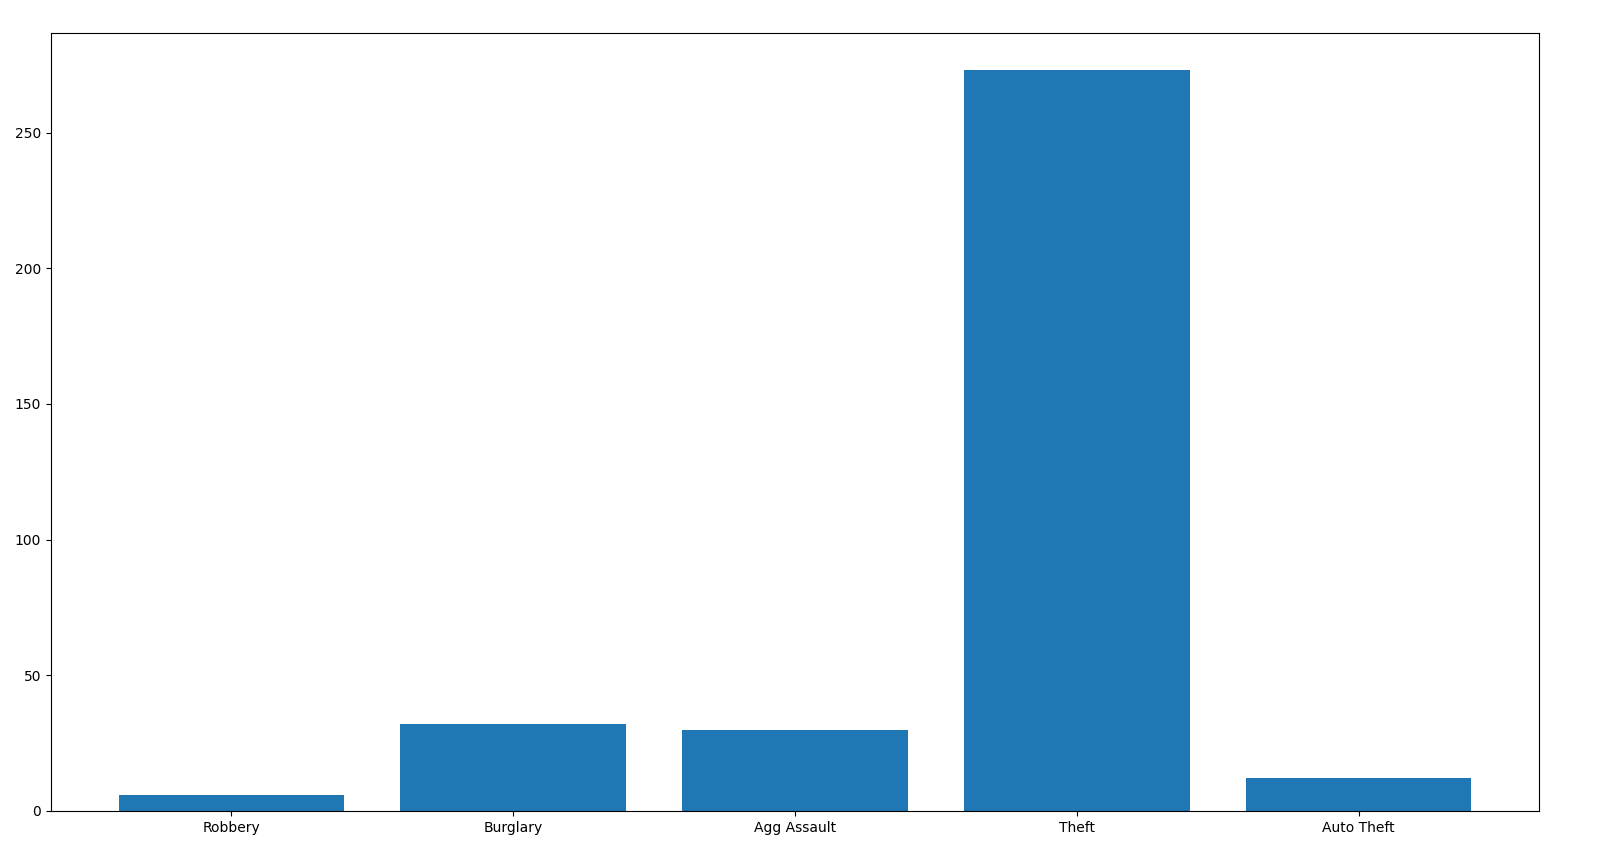
\includegraphics[width=0.9\textwidth]{figures/slaughter_lane.png}
  \caption{Četnosti zločinů na ulici Slaughter lane}
\end{figure}

\begin{thebibliography}{50}

\bibitem{dataset-source}
City of Austin \textit{2018 Annual Crime} [online, cit. 2021-12-28]
Dostupné z: \url{https://data.austintexas.gov/Public-Safety/2018-Annual-Crime/pgvh-cpyq} 
City of Austin, 6. leden 2020

\end{thebibliography}

\end{document}

